\section{Remote Vision Virtual Subsystem}%
\label{sec:remote-visi-subsyst-design}
The design specification devised in
Section~\ref{sec:remote-visi-subsyst-design} can now be implemented to the
target platform to fulfill the remote vision and telemetry functionalities
required. In this section the relevant implementation details are
addressed on the hardware and software domains.
%
\subsection{Hardware}%
\label{sec:hardware-rvvs-implem}
In the design stage, and in the first iterations of the
implementation, it is perfectly reasonable to adopt general domain environments,
such as virtual machines. Nonetheless, one must keep in mind that, ultimately,
the devised software will be running on hardware nodes. Thus, an important implementation step is the selection of the target
platform, taking into considerion several design criteria, such as, throughput,
memory footprint, storage, response time, connectivity, etc.

An example of a viable platform is the Raspberry Pi Zero W (Fig.~\ref{fig:pi-zero-w}), which is a low cost
board design (it retails for about 5 EUR) around the Broadcom system on-chip (SoC) BCM2835, which includes a
1 GHz single-core ARMv6 CPU, with a 64-bit architecture, allowing it to run
the full range of GNU/Linux distribution. Among other resources, it includes 512
MB RAM, VideoCore IV GPU, 40 GPIO pins, mini HDMI and micro-USB ports,
\gls{csi} connector, Micro SD Card Slot and on-board Bluetooth Low Energy (BLE)
4.1 and Wi-Fi based.

The Raspberry Pi Zero W provides the required communications
(Bluetooth and Wi-Fi) and camera interfaces, on a fully-fledged environment
capable of running 64-bit OS and at low cost, thus, making it
suitable for the implementation. Additionally, it packs in a small form-factor,
even with the inclusion of the camera, as illustrated in
Fig.~\ref{fig:pi-zero-w-cam}. The camera module has several models ranging from
5 to 12 megapixel resolution with high quality video capture (up to 1080p30) in
the 20--35 EUR pricepoint.
%
% Pi Zero W
\begin{figure}[!hbt]
\centering
    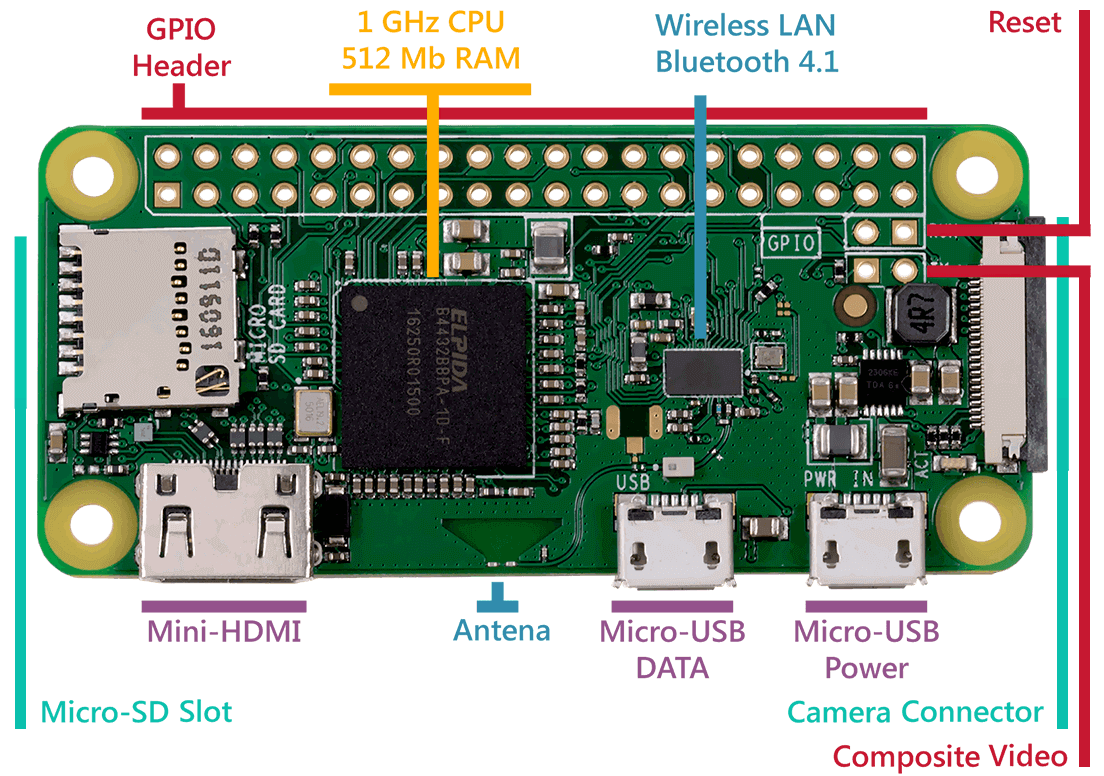
\includegraphics[width=0.6\textwidth]{./img/pi-zero-w.png}
  \caption{Raspberry Pi Zero Wireless overview}%
\label{fig:pi-zero-w}
\end{figure}
% Pi Zero W Camera
\begin{figure}[!hbt]
\centering
    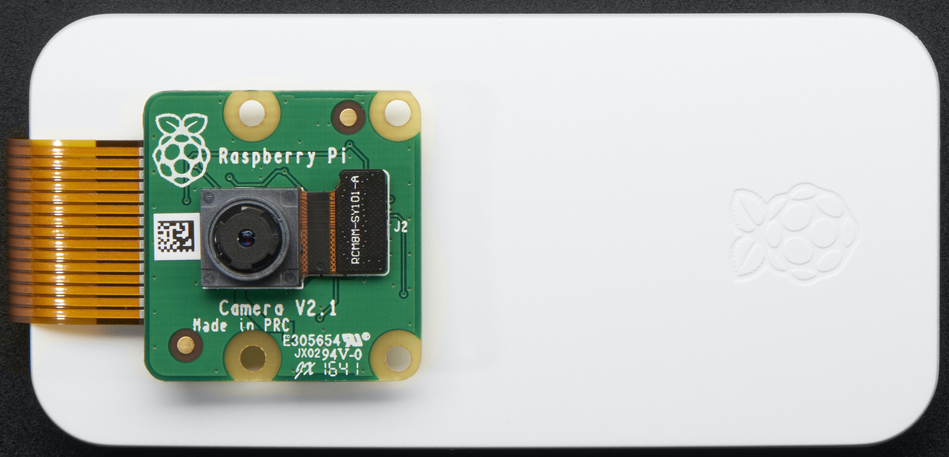
\includegraphics[width=0.6\textwidth]{./img/pi-zero-w-cam.jpg}
  \caption{Raspberry Pi Zero Wireless overview}%
\label{fig:pi-zero-w-cam}
\end{figure}
%
%
%%% Local Variables:
%%% mode: latex
%%% TeX-master: "../../../dissertation"
%%% End:
